\documentclass{article}
\usepackage{tikz}

\begin{document}

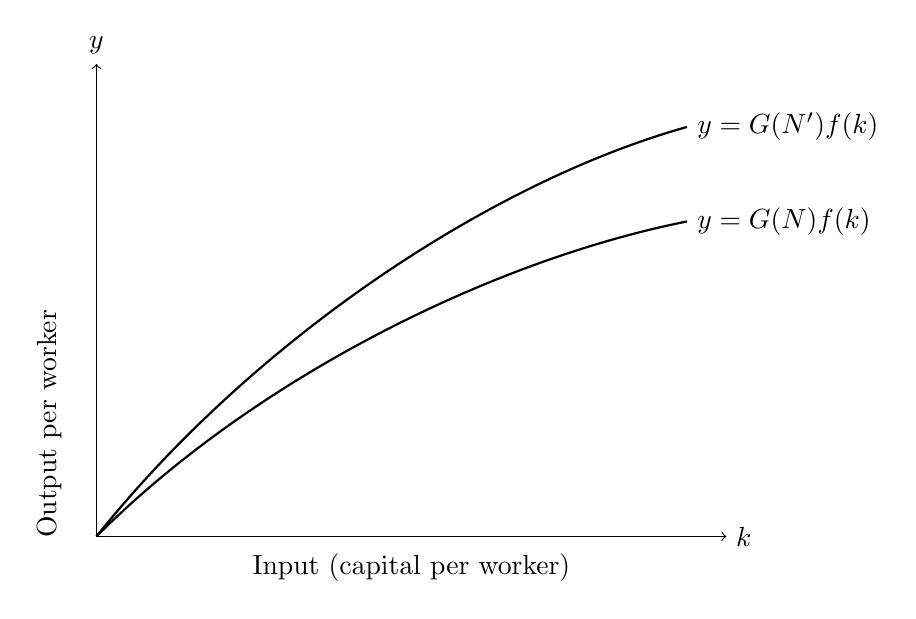
\begin{tikzpicture}
% Axes
\draw [->] (0,0) -- (8,0) node[right]{$k$}; 
\node [below] at (4,-0.1) {Input (capital per worker)};
\draw [->] (0,0) -- (0,6) node[above]{$y$};
\node [align=center, left, rotate=90] at (-0.6,3) {Output per worker};

% Production functions
\draw[thick] (0,0) .. controls (2,2) and (5,3.5) .. (7.5,4) node[right]{$y=G(N)f(k)$};
\draw[thick] (0,0) .. controls (2,2.5) and (5,4.5) .. (7.5,5.2) node[right]{$y=G(N')f(k)$};
\end{tikzpicture}

\end{document}